\documentclass[letter, article]{article}
\usepackage{graphicx}
\usepackage{parskip}
\usepackage{lipsum}
\usepackage[hidelinks]{hyperref}
\usepackage[left=2cm,top=1.5cm,right=2cm,bottom=1.5cm]{geometry}

\begin{document}

\begin{titlepage}
	\centering
	% \includegraphics[width=0.15\textwidth]{example-image-1x1}\par\vspace{1cm}
	{\scshape\LARGE Golden Phoenix \par}
	\vspace{1cm}
	{\scshape\Large Robot Design Overview\par}
	\vspace{1.5cm}
	{\huge\bfseries \par}
	\vspace{2cm}
	{\Large\itshape Alex Bellock, Justin Spielman, Jacob Livoni, Ashely Gordon, Jared Sabila, Jason Soler, and Hadyn Tibbs\par}
	\vfill
	supervised by\par
	Kenneth E. Bellock

	\vfill

% Bottom of the page
	{\large \today\par}
\end{titlepage}

\section{Software Example}

\begin{center}
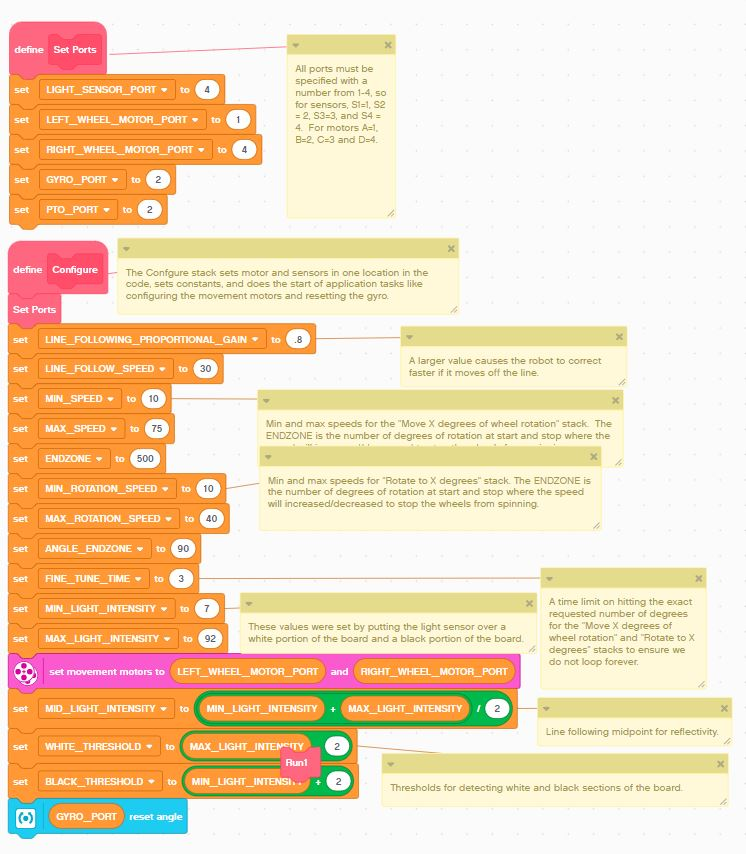
\includegraphics[width=0.20\textwidth]{ConfigureStack}
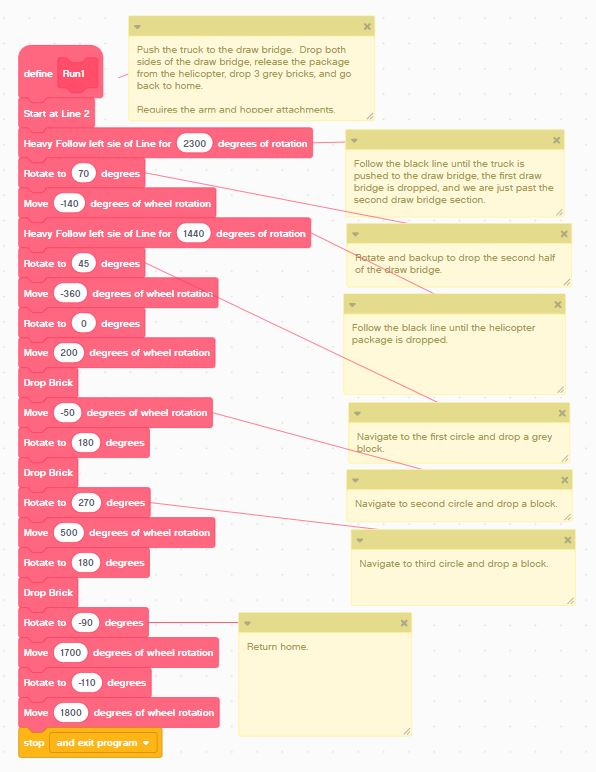
\includegraphics[width=0.20\textwidth]{Run1}
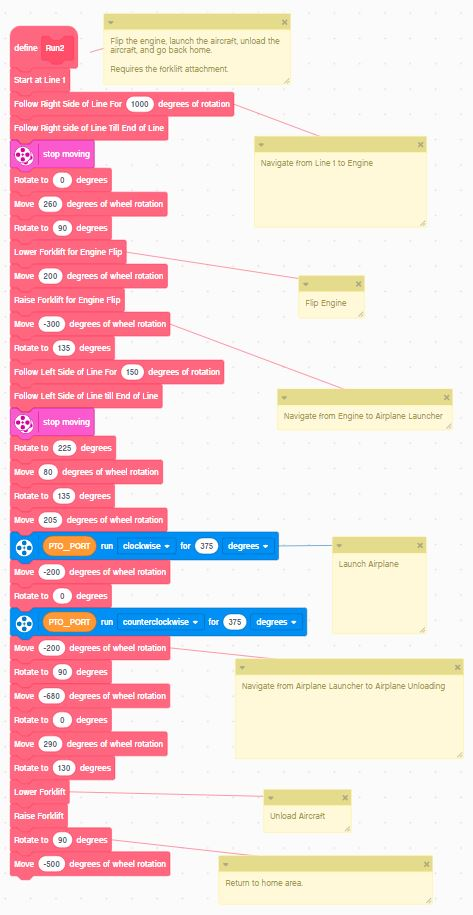
\includegraphics[width=0.20\textwidth]{Run2}
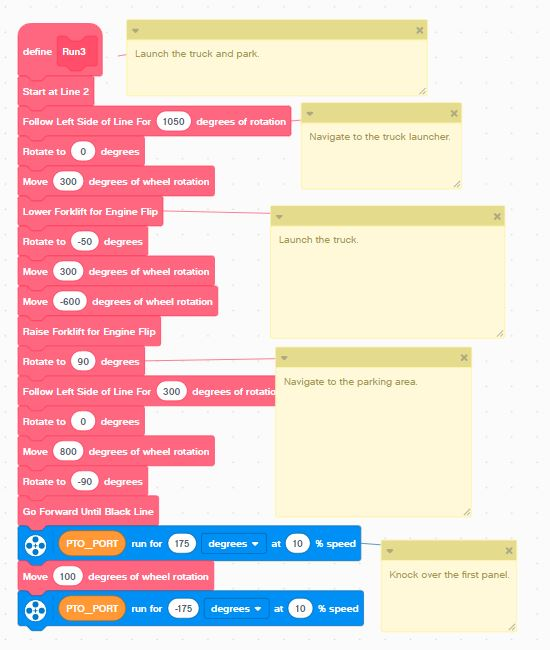
\includegraphics[width=0.20\textwidth]{Run3}
\end{center}

\begin{center}
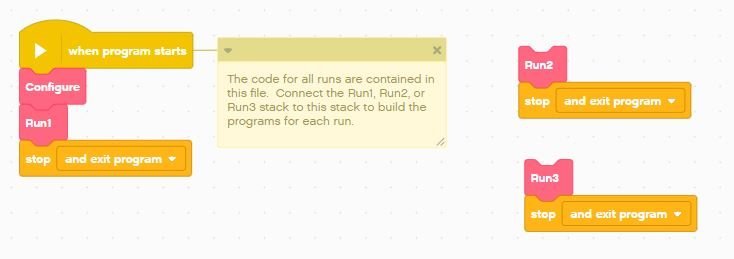
\includegraphics[width=0.30\textwidth]{Main}
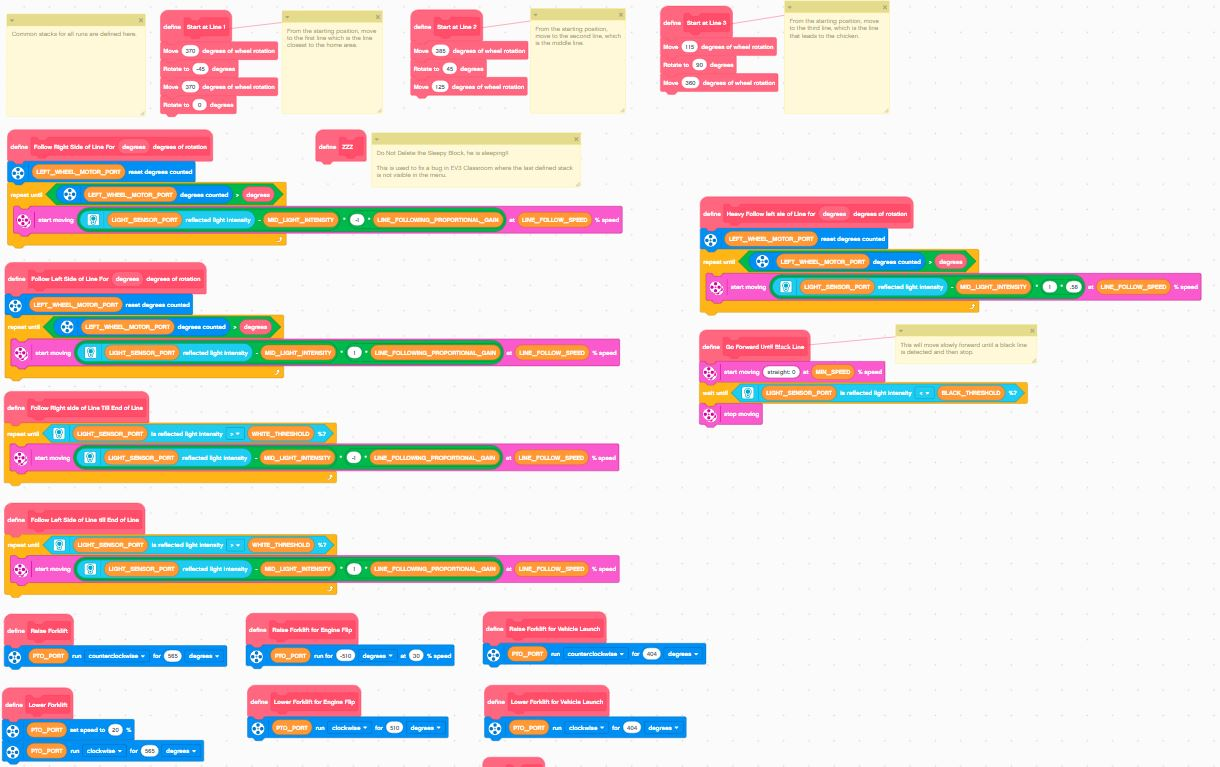
\includegraphics[width=0.30\textwidth]{Common1}
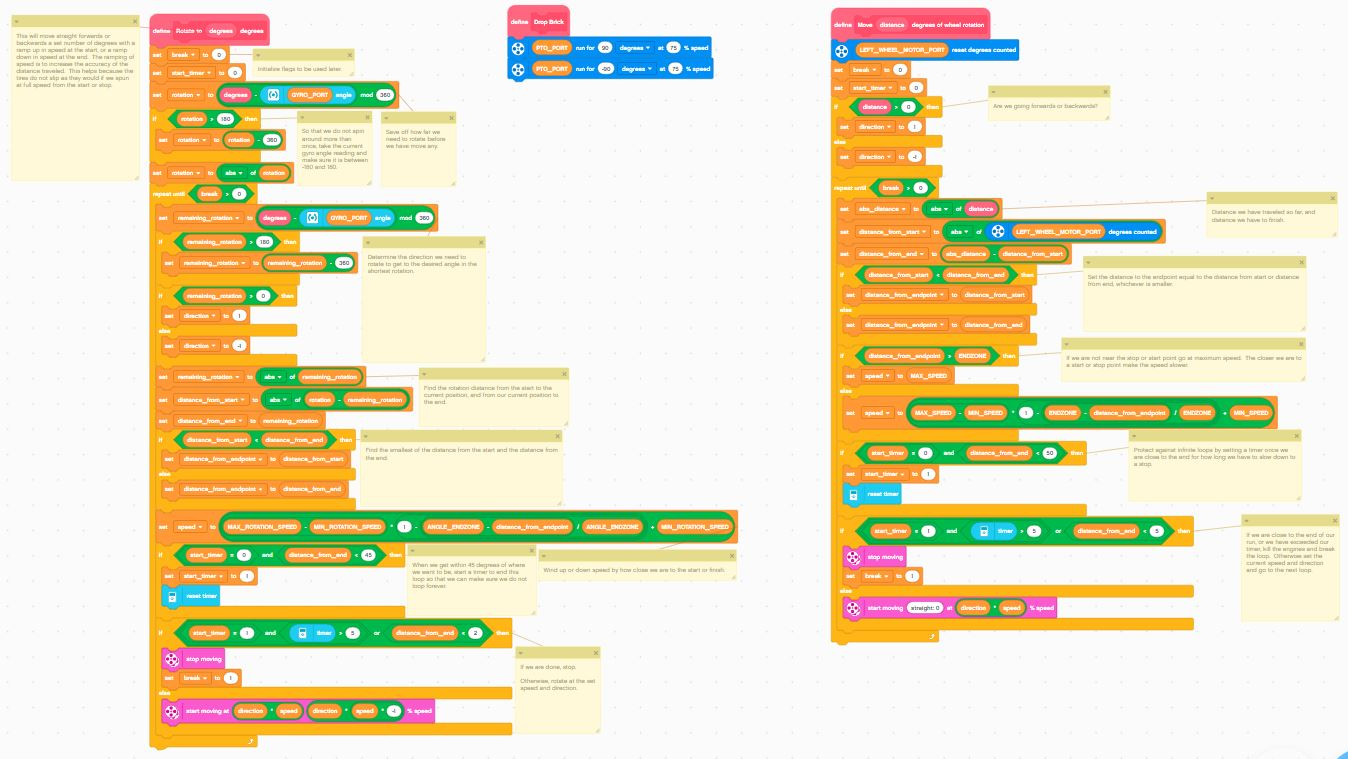
\includegraphics[width=0.30\textwidth]{Common2}
\end{center}

\section{Robot and Attachments}

\subsection{Base Robot}

The base robot for the Golden Phoenix team was derived from the COR3 robot plans by Michael Buss Andersen, found at \url{https://flltutorials.com/en/robotgame/building/one%20kit%20build/2018/06/12/COR3.html} and is shown below.

\begin{center}
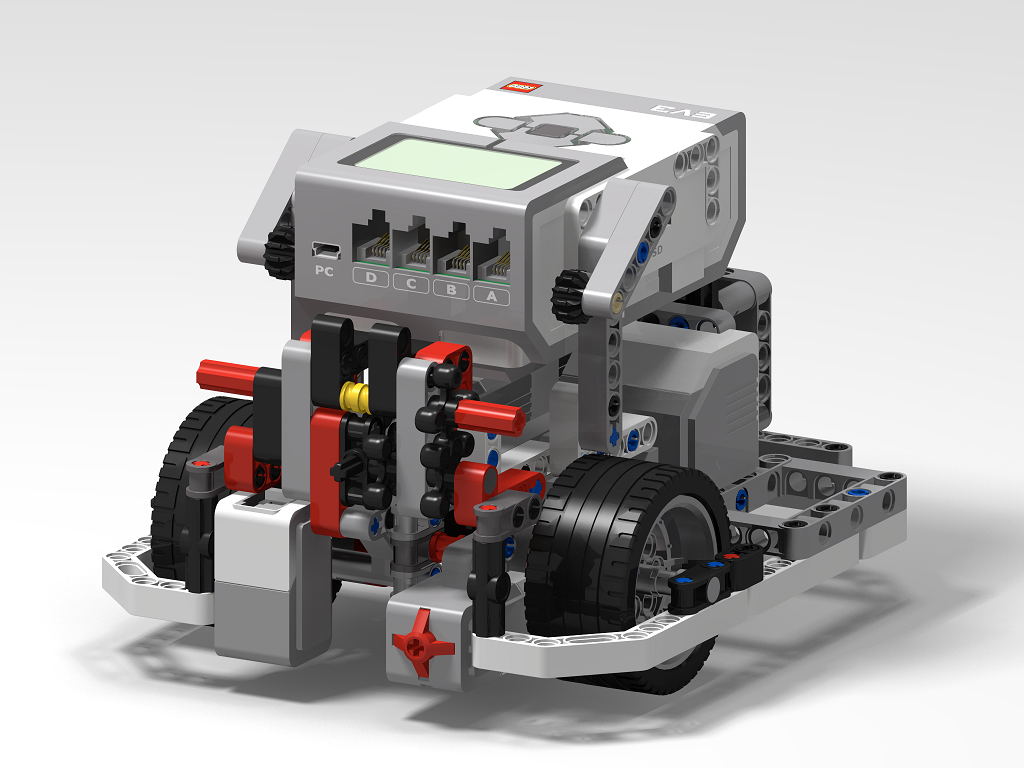
\includegraphics[width=0.75\textwidth]{COR3}
\end{center}

The side rails were removed, as well as the touch sensor, a gyro sensor was added to the top and the gearing was modified to add lifting power to the forklift attachment described below.  The resulting robot is shown below and was the base to which all attachments were designed to complete the missions.

\begin{center}
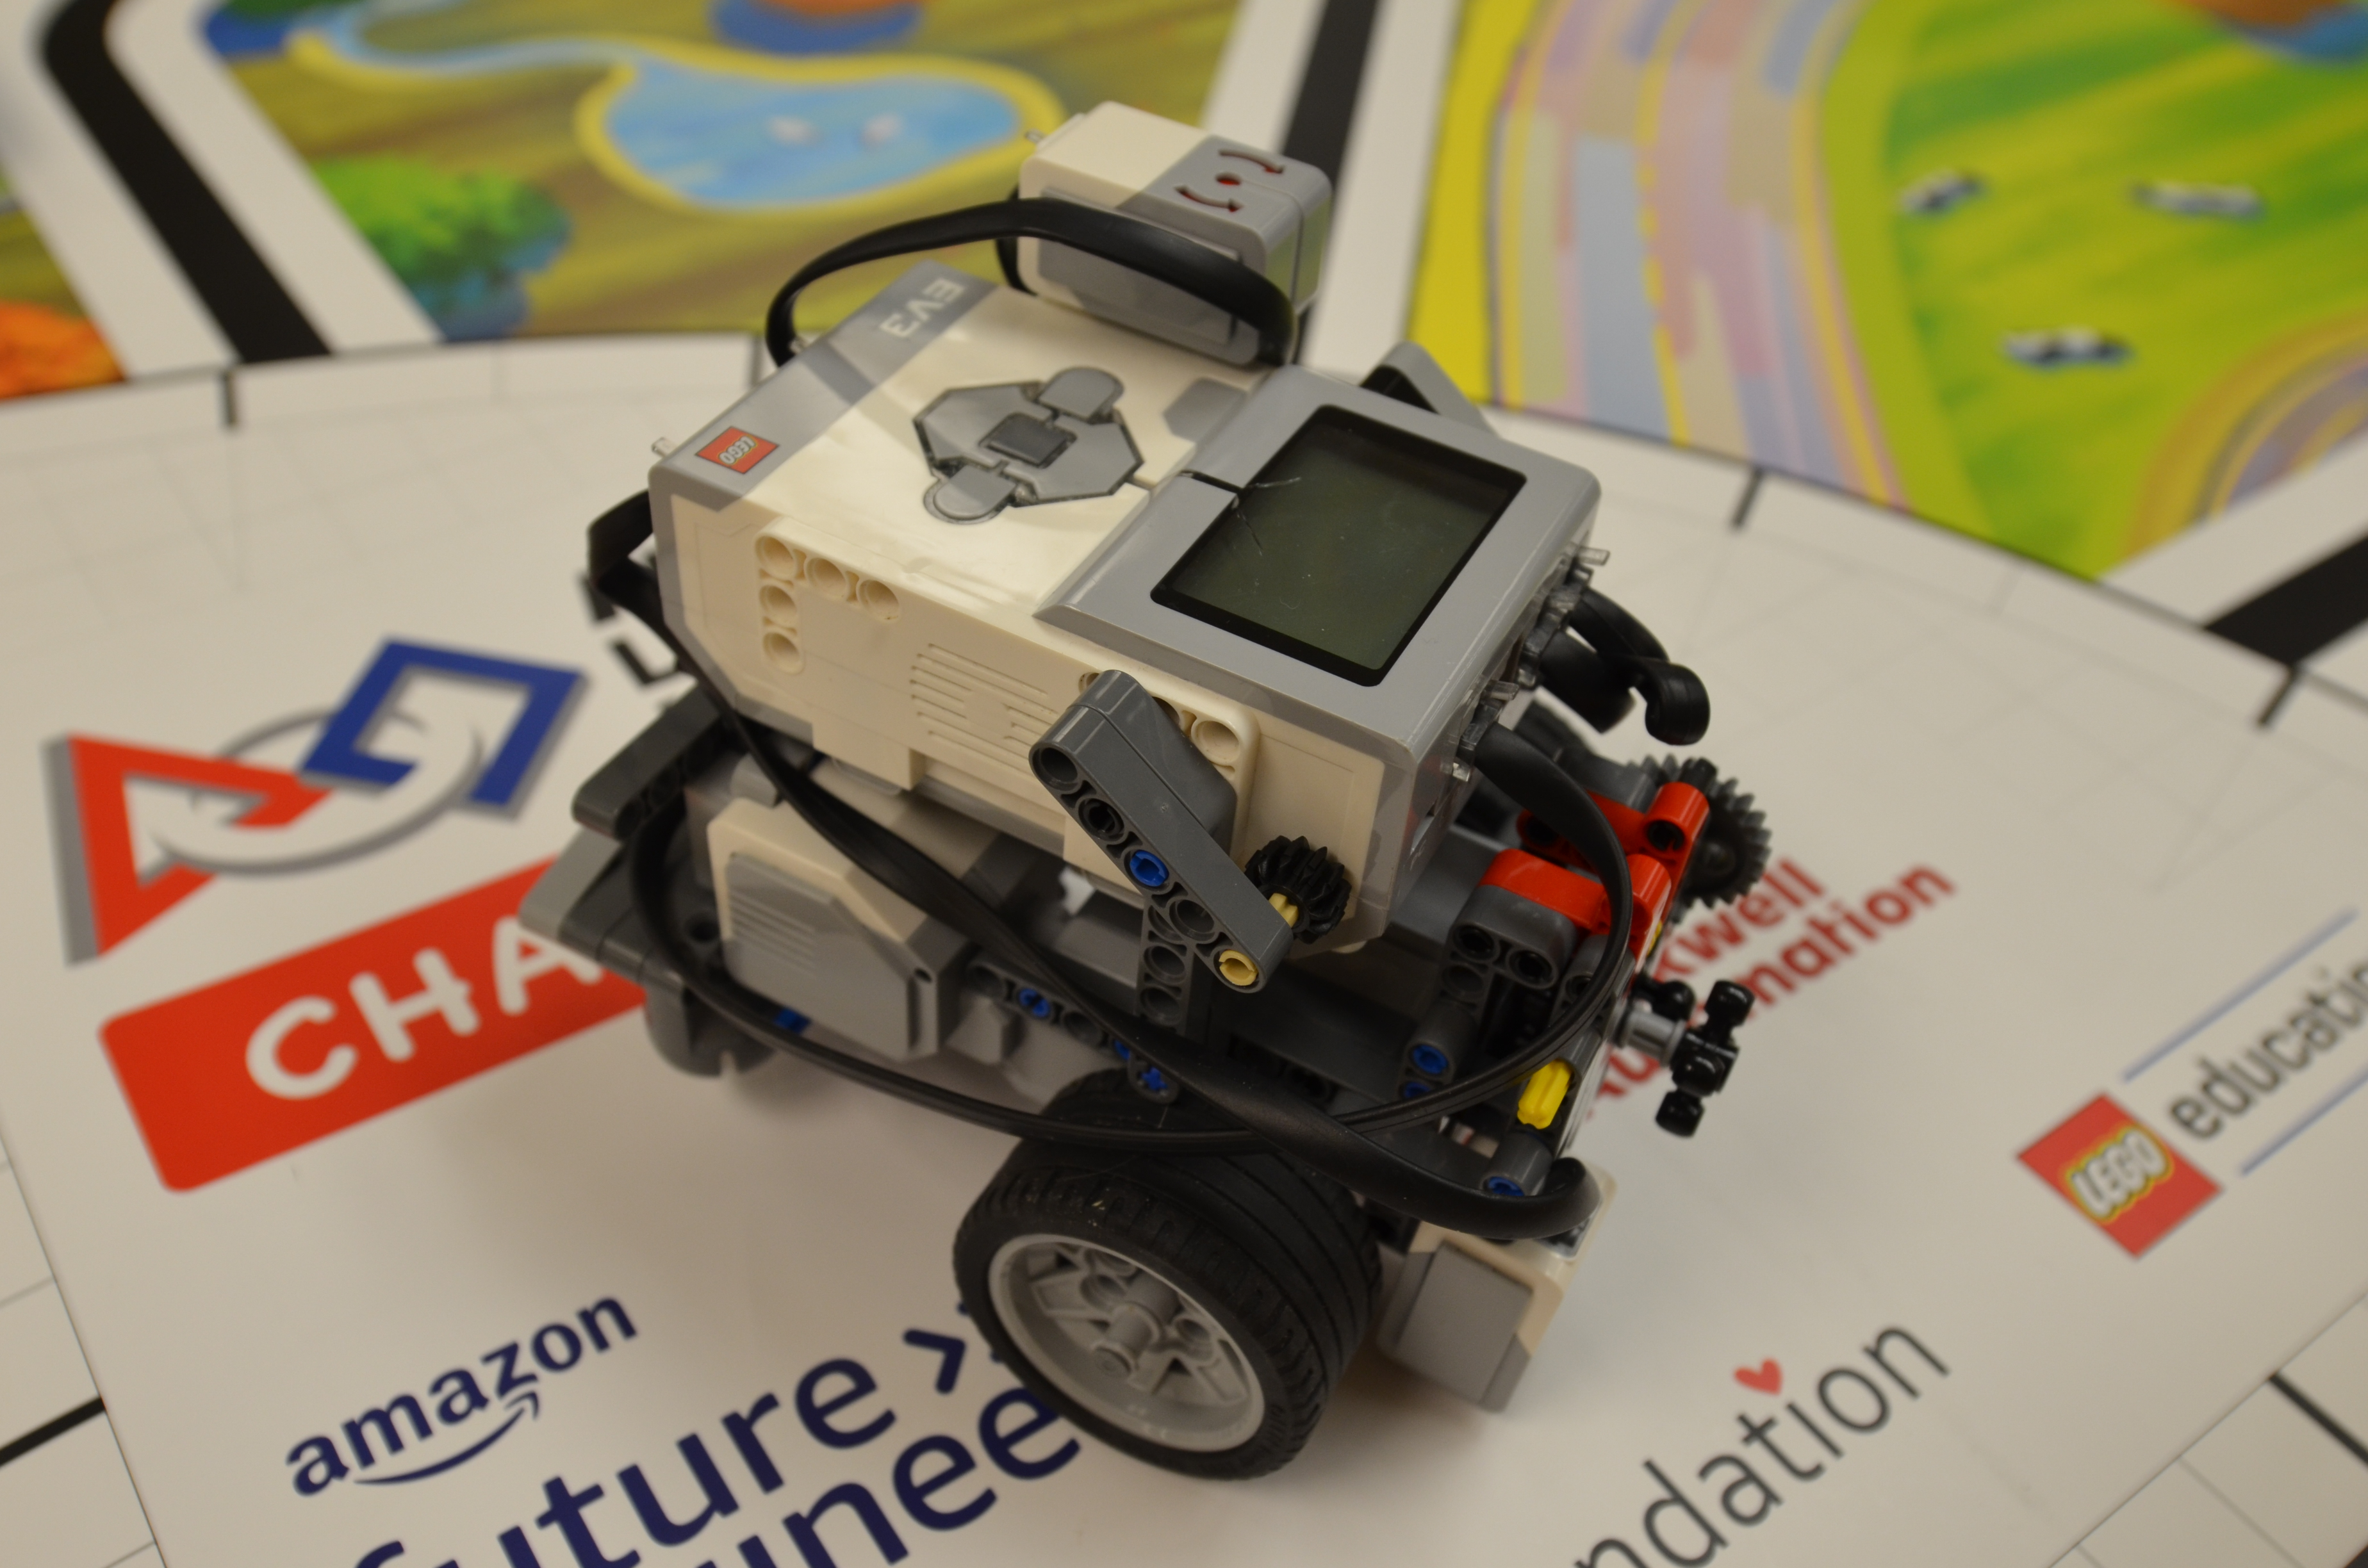
\includegraphics[width=0.48\textwidth]{DSC_3895}
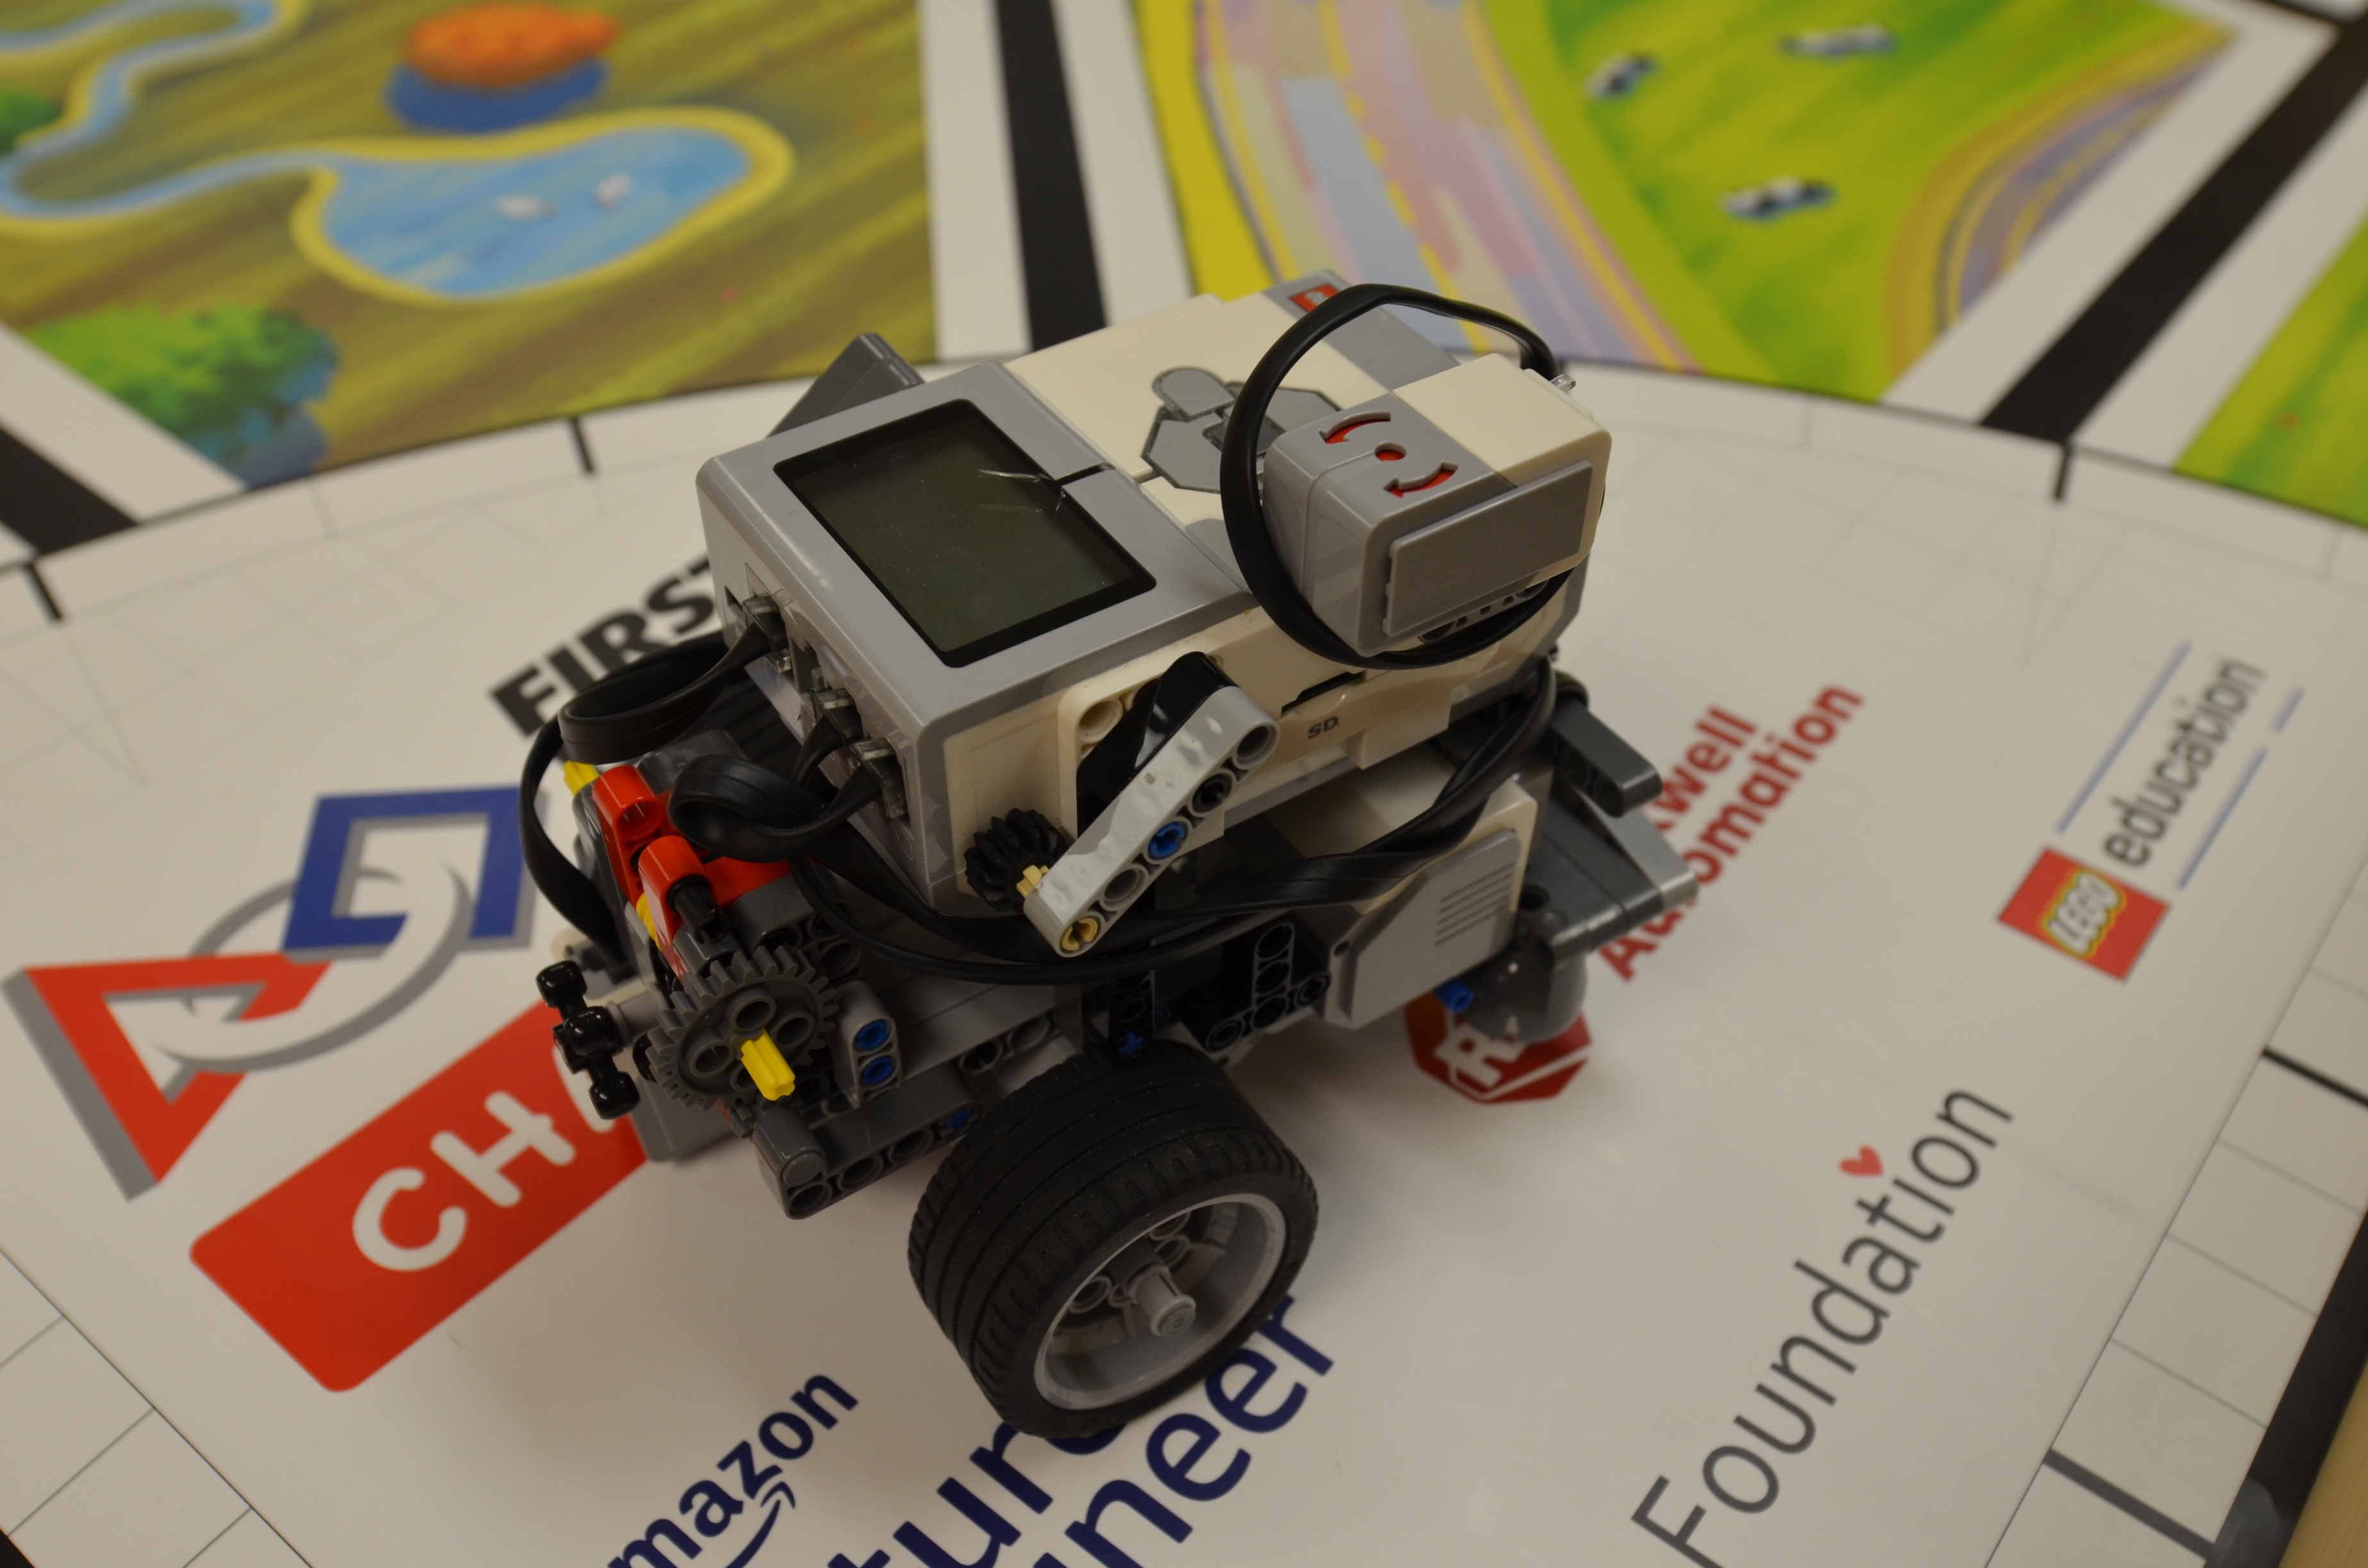
\includegraphics[width=0.48\textwidth]{DSC_3896}
\end{center}

\subsection{Attachments}

Attachments were built to complete the missions, and were added to the base robot.  The following sections describe each of the attachments.

\subsubsection{Forklift}

The forklift was used to lift and move items.  It rotates up to a stowed position and then can be used to press down, lift up, or push things around on the game board.  The forklift is shown in the high position below.

\begin{center}
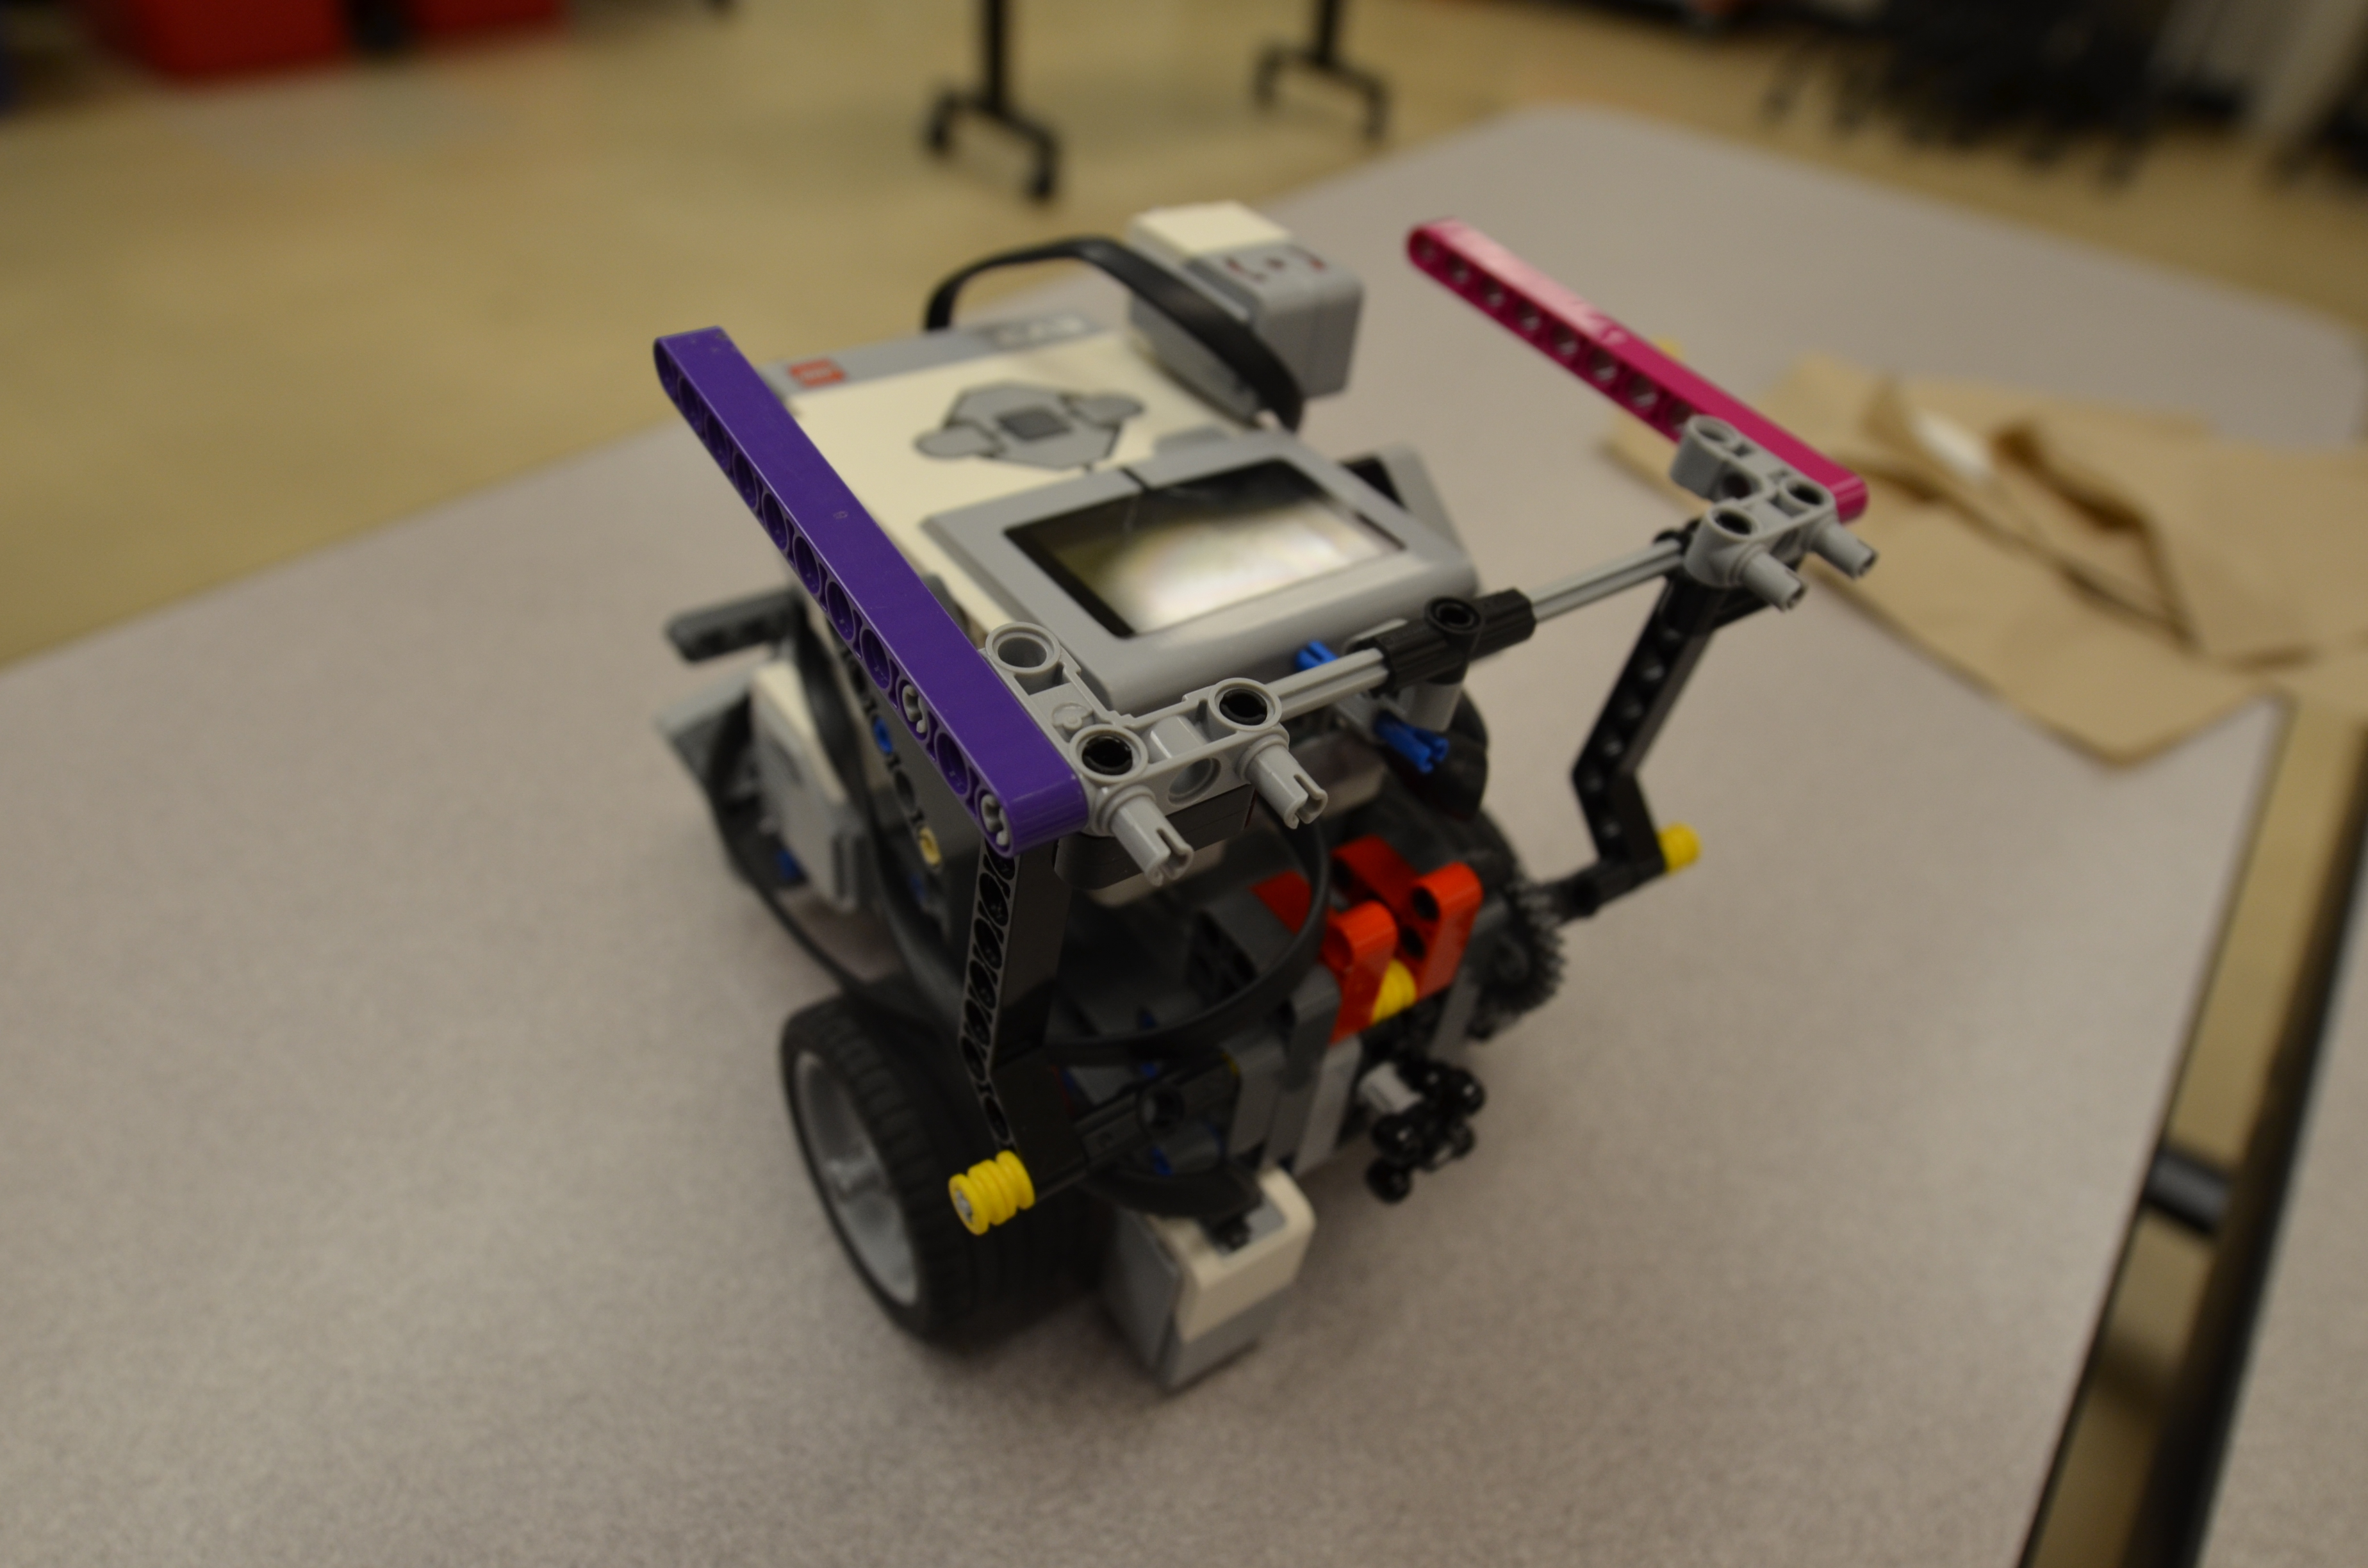
\includegraphics[width=0.75\textwidth]{DSC_3883}
\end{center}

\subsubsection{Hopper}

The hopper was used to place bricks in the circles around the table.  The hopper has an arm on the bottom which is rotated to drop and brick and push it out onto the game board.  It is shown in the picture below.

\begin{center}
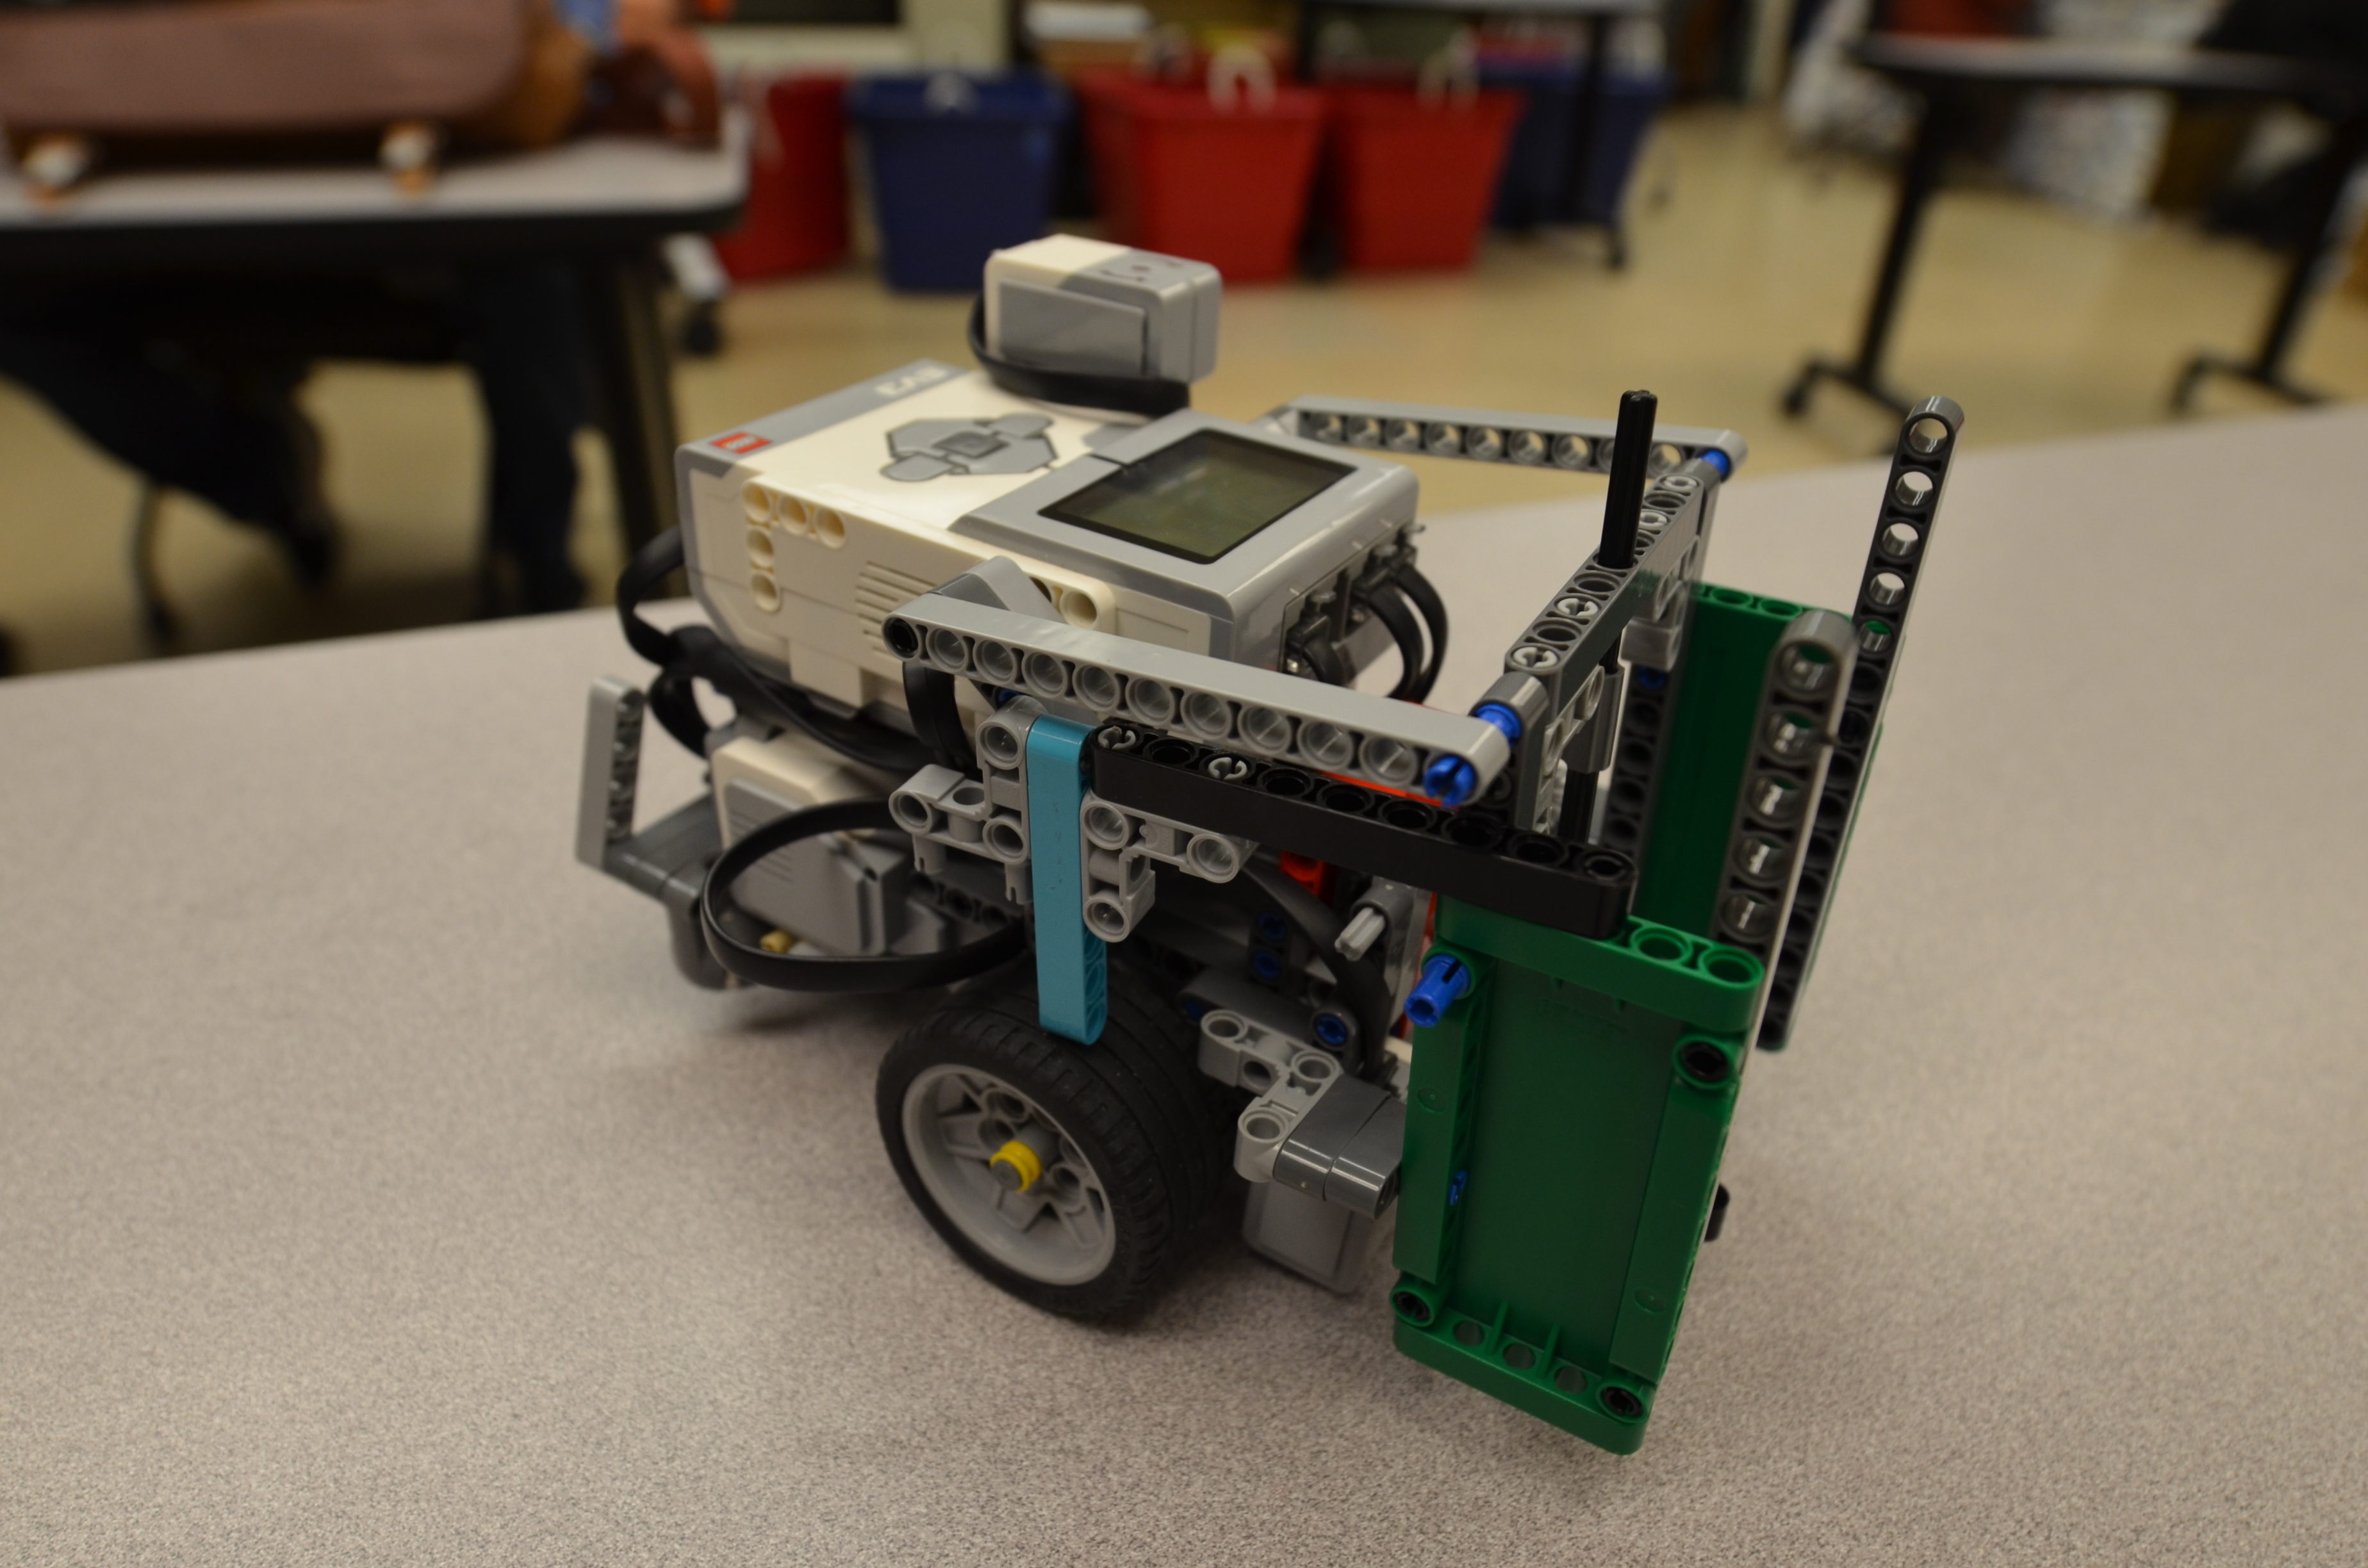
\includegraphics[width=0.75\textwidth]{DSC_3880}
\end{center}

\subsubsection{Arm}

The arm attachment was used to push things on the game board like the truck and the draw bridge.  It is shown fully extended in the following image.

\begin{center}
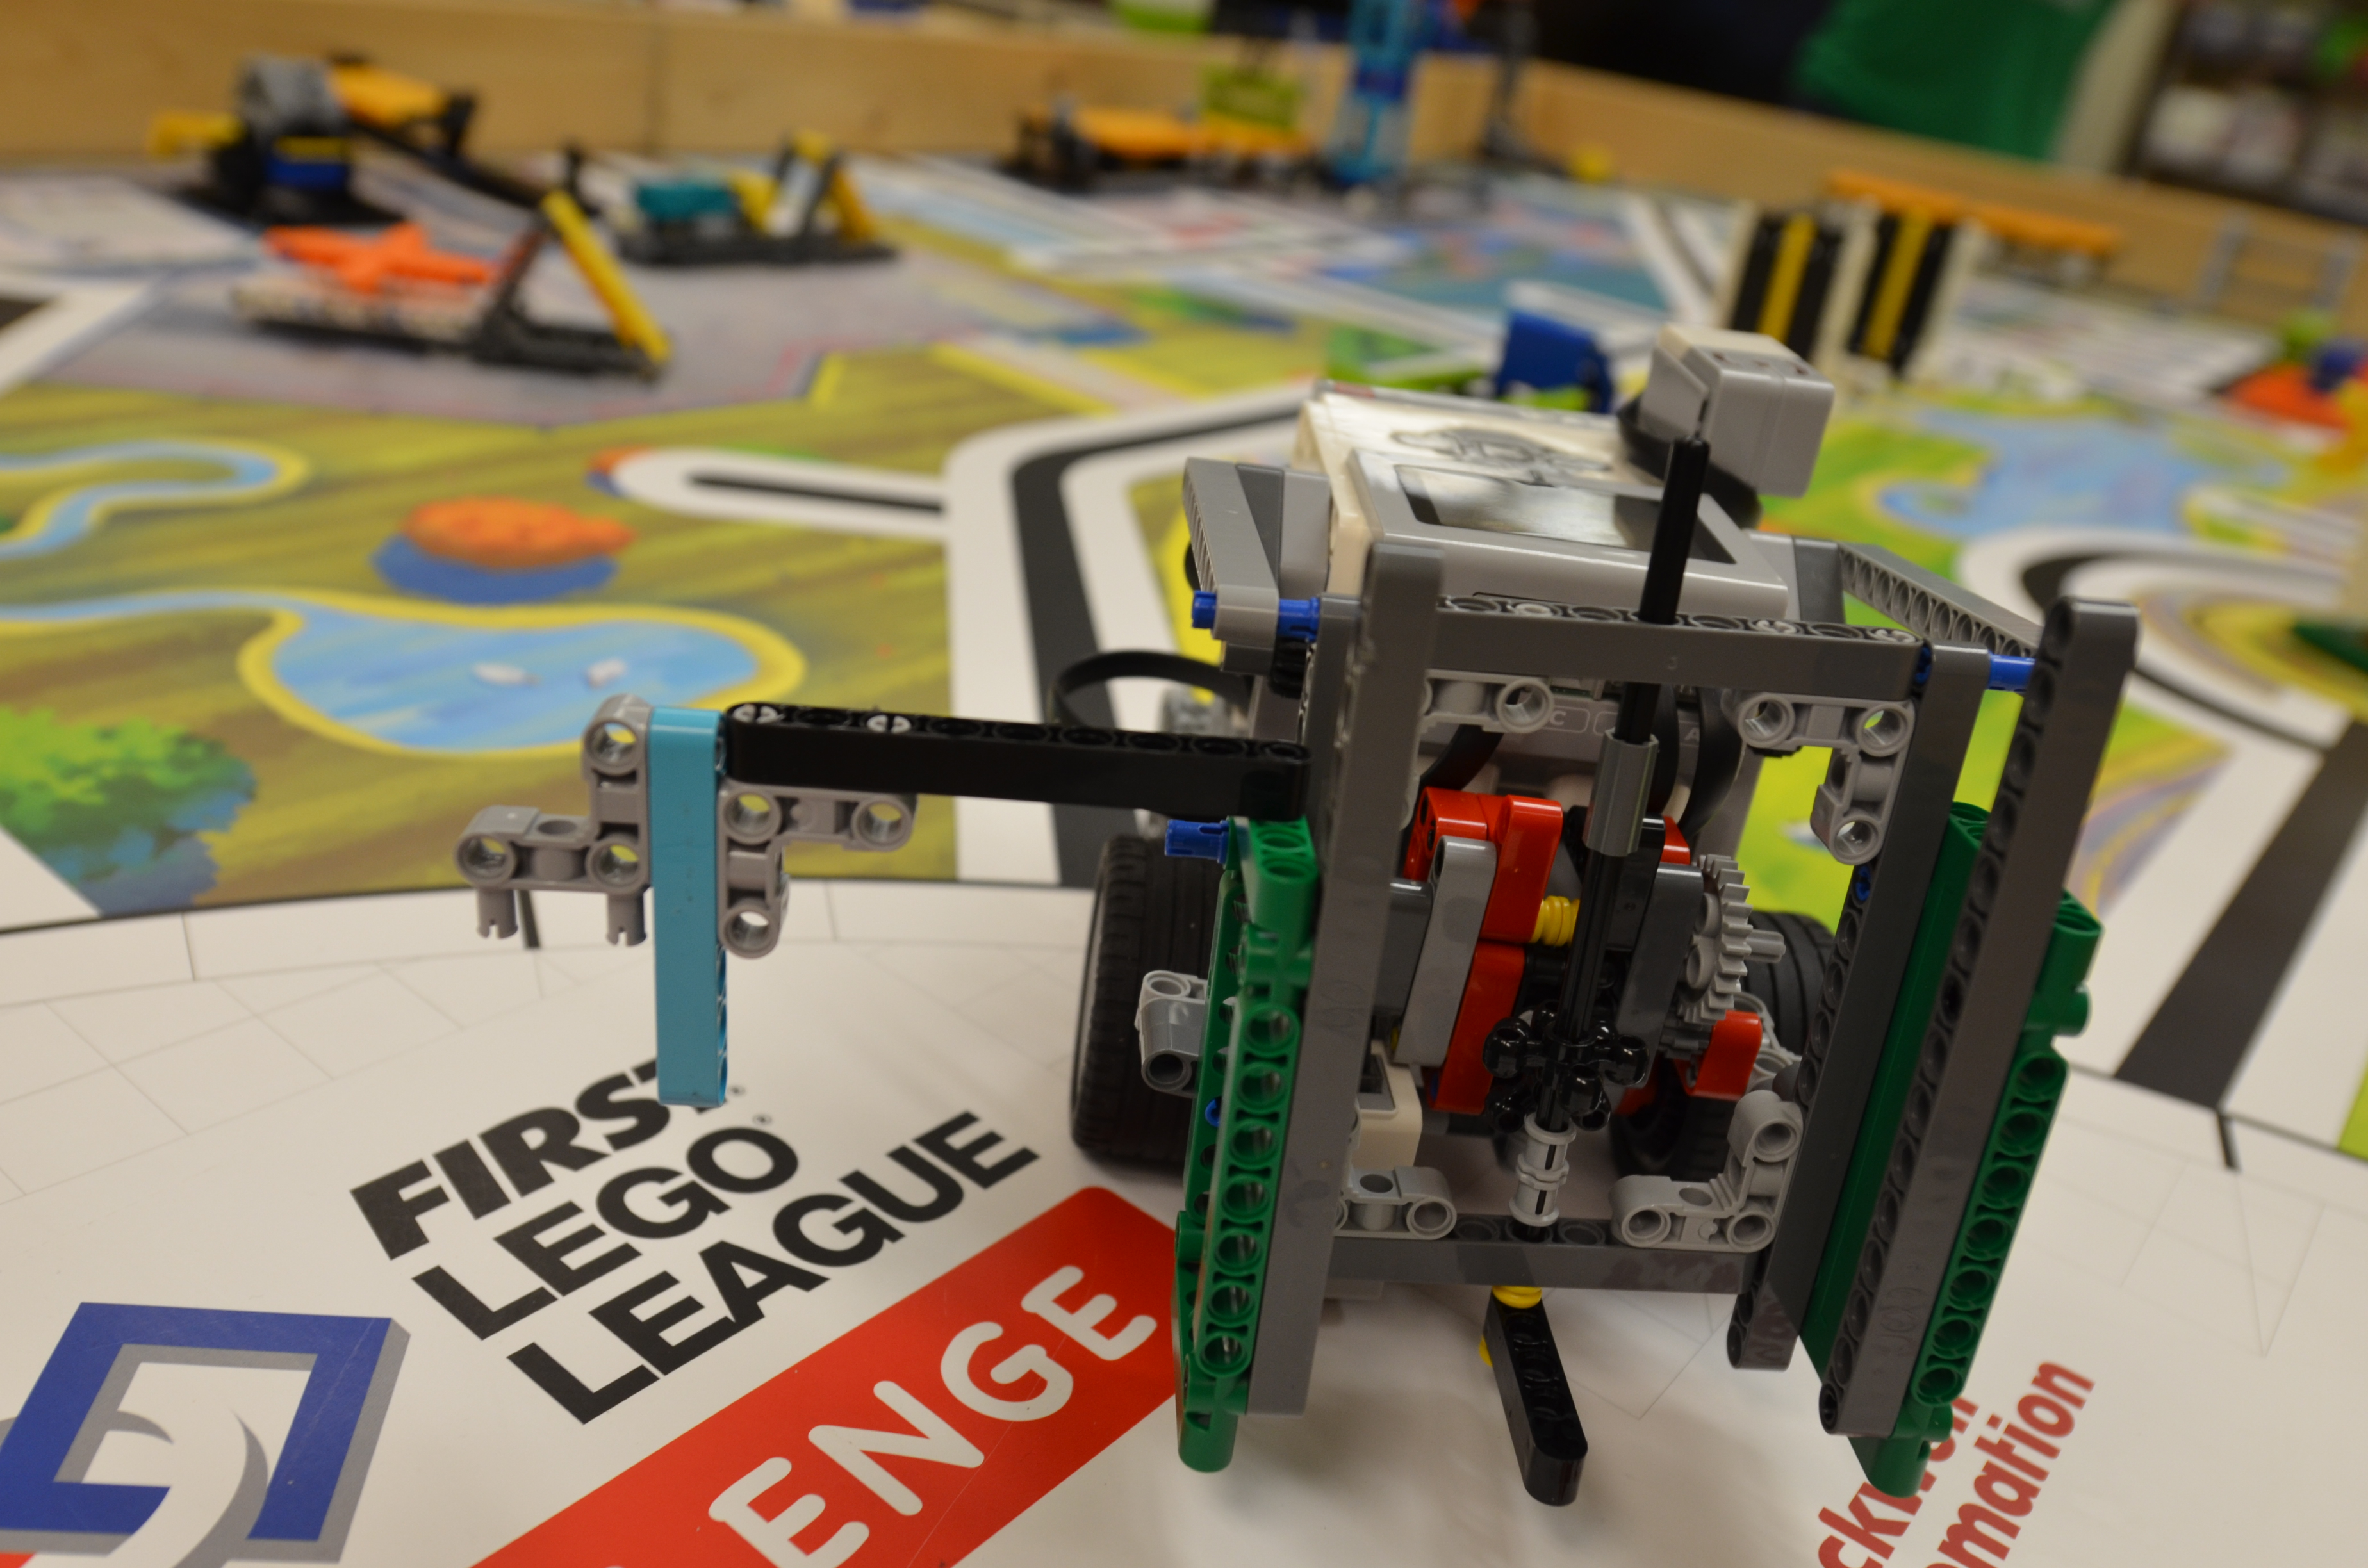
\includegraphics[width=0.75\textwidth]{DSC_3898}
\end{center}

\section{Mission Strategy}

The mission strategy was to use as many of the sensors in our code to make moving around the board more repeatable and accurate.  Runs were designed on the board, to use an attachment and complete a series of missions.  Each of the runs are described in the following sections.

\subsection{Run 1}

Run 1 is configured with the hopper -- loaded with three grey bricks, and the arm attachment.  We start off by line following the middle line to the truck and using the arm to push it to the hook on the draw bridge, and then push over the first half of the drawbridge.  Then we move forward till we pass the second half of the drawbridge, and then back up to knock it down.  We then continue to line follow to drop the helicopter package.  Then we navigate to the circles on the far side of the board, and drop the three grey bricks in the circles.  We then return the home area.

\subsection{Run 2}

Run 2 is configured with the forklift.  We start by line following the left line until its left hand turn, and then navigate to the engine and flip it over.  Then the robot turns and uses the forklift attachment to grab and pull the airplane from the launcher past the line.  Then the cargo plane is unloaded, and we drive back to the home area.

\subsection{Run 3}

Run 3 is configured as in Run 2.  We line follow the middle line until we are alongside the truck launcher.  We then approach the truck launcher from the side, and lower the forklift and push the truck past the launch line.  The robot travels back to the line follows it for a short distance and then turns towards the parking area.  Once at the parking area, the light intensity sensor is used to position the robot on the black line and then the fork lift is lowered to push over the yellow barrier.  That ends run 3.

\section{Design Process}

The design process started by planning out each of the runs described above.  The capabilities needed were then identified, like line following and raising and lowering of the forklift. We then designed common blocks for each of these capabilities, and then strung them together into code stacks for each of the runs.  Part of the team worked on designing the attachments, and then worked with other members of the team on paring the attachments to code that would use those attachments.

\end{document}
